\documentclass[final,1p,12pt]{elsarticle}

%% The amssymb package provides various useful mathematical symbols
\usepackage{amssymb}
%% The amsthm package provides extended theorem environments
\usepackage{amsthm}
%% The amsmath package provides binomial notation for us
\usepackage{amsmath}
% The tikz package provides drawings for Combinations set notation (Venn Diagram), and later on graphs.
\usepackage{tikz}
% The pgfplots package provides an extended environment for graphing.
\usepackage{pgfplots}

%% Removes the wonky "Preprint Submitted to Elsevier" and adds a front-page footer. 
\makeatletter
\def\ps@pprintTitle{%
 \let\@oddhead\@empty
 \let\@evenhead\@empty
 \def\@oddfoot{\centerline{\thepage}}%
 \let\@evenfoot\@oddfoot}
\makeatother

%% Definitions
\newtheorem{definition}{Definition}
\newtheorem{example}{Example}
\newcommand*\mean[1]{\bar{#1}}
\newcommand*\median[1]{\tilde{#1}}
\pgfplotsset{compat=1.13}
\usetikzlibrary{backgrounds}
%% Start of Document
\begin{document}

%% Header
\begin{frontmatter}
    \title{Exam Notes for MDM4UI}
    \author{John Oss\\
            \today\\
            \LaTeX}
    \begin{abstract}
        Notes for all topics taught in MDM4UI (Data Management) from the winter term of the 2016-2017 school year at GCI.  
        Please refer to the appendix for a walk-through of example questions that will probably be on the exam. 
        Sorry for the formatting. I'm not quite done yet.
    \end{abstract}
\end{frontmatter}

%% Table of Contents
%% TODO: After everything is finished, allow hyperlinking in the Table of Contents.
%%
%% \tableofcontents

%% Body
%% Sections are their own files to make debugging a lot easier.

\section{Permutations}

    \subsection{What are Permutations?}
    Permutations are the arrangements of objects in a set order. 
    For instance, how many ways can you rearrange the letters in the word "APPLE",
    or how many ways can you bring 4 people out of 20 friends to a party?

    \subsection{Factorial Notation}
    Often in permutations, we need to multiply descending consecutive numbers.
    Since these numbers are descending and not ascending, we can safely assume that \textbf{every factorial must be positive}. 
    For instance,  $5\cdot4\cdot3\cdot2\cdot1$ can often be simplified and written as \textbf{5!}, or 5 factorial.\\
    The general rule for factorial notation is: 
    \begin{equation*}%Factorial Equation
        n! = n\cdot(n-1)\cdot(n-2)\cdots3\cdot2\cdot1
    \end{equation*}
    The exception to this rule is 0!, which in this case would be $0! = 1$, which would follow the same thinking as $n^0=0$.
    
    \subsection{Rule of Product and Rule of Sum}
    How many different results can one get from flipping a coin 3 times?
    You have 2 possibilities, heads or tails, and you flip it 3 times.
    Essentially, you have three groups of two, or $2\cdot3$ different results, which turns out to be $6$ different possible results.
    This is called the \emph{Fundamental Rule of Product} or the \emph{Counting Principle}
    \begin{definition}
        The Rule of Product states that if the $1^{st}$ action can be performed in n ways, and the $2^{nd}$ action can be performed in m ways.
        They can be performed together in $n\cdot m$ ways. 
    \end{definition}
    What happens if the actions cannot be performed together? Such as which car to buy? In that case we have another rule, known as the \emph{Rule of Sum}.
    \begin{definition}
        The Rule of Sum states that if the $1^{st}$ action can be performed in n ways, and the $2^{nd}$ action can be performed in m ways, and these actions cannot occur together, then there are $n+m$ ways for either of the actions to occur.
    \end{definition}
    
    \subsection{N-Arrangements}
    Let's say you have 5 people, and you need to arrange them in a line.
    You put one person in the first spot, and now you have 4 left. Repeat this until you are left with one person, which fits into the last spot.
    You can express this mathematically by writing out $5!$ .\\
    This is quite similar to the Rule of Product as:
    \begin{enumerate}
        \item Each placement is a choice
        \item The number of choices is reduced with each previous action. 
    \end{enumerate}
    A permutation of \emph{n} objects is an arrangement of the objects in a \textbf{definite order}.
    This can be expressed with permutation notation, shown below where P(n,n) equals the number of ways to permute n objects.
    \begin{equation*}
        P(n,n) = n!
    \end{equation*}
    This equation will only work when the number of spaces to occupy and the number of objects are equal.
    In other cases we'll have to use an r-arrangement.
    
    \subsection{R-Arrangements}
    If you have more objects than places you can put the objects into, then we can use something called an r-arrangement.
    An r-arrangement is a permutation of \emph{n} objects taken \emph{r} at a time, as is shown below.
    \begin{equation*}
       P(n,r) = \frac{n!}{(n-r)!} 
    \end{equation*}
    Where $P(n,r)$ equals the total number of arrangements you have, divided by the number of unused objects.
    This is most commonly displayed on calculators as \emph{nPr}.
    For example you have 4 subjects, but you can only study two at a time.
    The equation for that would be $\frac{4!}{(4-2)!}=12\mbox{ combinations.}$ 
    
    \subsection{Permutations with Repeating Elements}
    All previous examples will ONLY work with non-repeating elements, such as the letters in the word "MONTREAL", or 5 different books.
    They will definitely NOT work for questions with repeating elements, such as the word "FIJI".
    For all repeating elements we'll have to follow another rule shown below.
    \begin{definition}
        In general, the number of arrangements of \emph{n} objects of which \emph{a} of one kind are alike, and \emph{b} of one kind are alike and so forth is given by the expression below, Where the number of permutations can be found by dividing the total number of possible combinations by the repeating elements.
        \begin{equation*}
            \frac{n!}{a!b!c!\cdots}
        \end{equation*}
    \end{definition}
    
    \subsection{Problem Solving with Permutations}
    There are 3 methods for solving problems with permutations. They are called: the Indirect Method, the Case Method, and Circular Arrangements.
    
        \subsubsection{Indirect Method}
        The indirect method involves taking all possibilities and subtracting those which are not wanted.
        For instance, say you have 3 people that need to sit at a table, but 2 of them don't want to sit beside each other.
        There is a step-by-step process that you can use for this question that is explained below.
        \begin{enumerate}
                \item Find all possible permutations (ex. P(3,3) ),
                \item Find all unwanted permutations (in this case when they are together),
                \item Subtract the unwanted permutations from the wanted permutations.
            \end{enumerate}
        This can be written as:
        \begin{equation*}
            \mbox{\textbf{Wanted Outcomes}} = \mbox{Total Outcomes}-\mbox{Unwanted Outcomes}
        \end{equation*}
    
        \subsubsection{Case Method}
        The Case Method involves breaking down the equation into manageable parts, then adding them to get the final solution.
        There is a step-by-step example problem in Section 1 of the appendix, along with an explanation of why, and how you manage the "breaking into parts" aspect.
    
        \subsubsection{Circular Arrangements}
        Circular arrangements are no longer a part of the curriculum, and as such they will not be tested on, but they are still quite useful to know in niche cases.
        If you have seven people seated at a table, and they all move to their rights, their positions may have moved, but their order remains the same, like a circle.
        Keep in mind that if there is some fixed point, the question just ends into a typical linear arrangement, with the equation simplifying to $1 \cdot (n-1)!$.

\section{Combinations}

    \subsection{What are Combinations?}
     A Combination is a way of selecting objects (permuting) from a group, without the order being important.
     In essence, it is orderless permutations. Let $ABC$ be a permutation.
     With permutations we asserted that $ABC$ and $BAC$ are different, as they are ordered differently.
     In combinations, we assert that $ABC$ and $BAC$ are the same, as they contain the same objects, just in a different order.

    \subsection{Set Theory}
    Set Theory involves the creation and manipulation of sets and their properties.
    A set is a collection of distinct objects in which their order does not matter.
    The objects in this set are called elements.
    If a set does not have any elements in it, we refer to it as a \emph{null set}, which is shown as $\emptyset$ or $(\emptyset)$.
    This null set is a subset of everything.
    If we want to describe a set containing elements, we must follow the example below.
    \begin{equation*}
        X = \{a,b,c,d,e,f,\cdots,y,z\}
    \end{equation*}
    If we wish to describe the number of elements in the set, we can use $n(X)$, where X represents the set, and n returns the number of elements in that set.
    In this case $n(X) = 26$, as set X contains all the letters of the alphabet.
    Sets are referred to differently when compared to other sets, as defined below.
    \begin{definition}
    Special Properties of Sets when Compared to Other Sets
    \begin{enumerate}
        \item If two sets have no elements in common they are called disjoint sets.
        \item If two sets have all elements in common they are equal.
        \item If all of elements of A are also in B then A is a subset of B $(A\subseteq B)$
    \end{enumerate}
    \end{definition}
    
        \subsubsection{Universal Set and Complement Sets}
        The set of all elements being considered is called the\emph{universal set} and is always denoted by $S$.
        When referring to a set of all elements that are in the universal set, but\textbf{ not in set A}, we call this the complement of $A$ or $A`$. For example:
        \begin{equation*}
            S = \{1,2,3,4\}, A = \{1,3\}, A`=\{2,4\}
        \end{equation*}
        
        \subsubsection{Unions and Intersections}
        For two sets of A and B, the \textbf{union} of A and B or $A\cup B$, is the set of all elements in A or B, not including duplicates.
        \begin{equation*}
            S = \{1,2,3,4\}, A = \{1,3\}, B =\{1,2\}, A\cup B=\{1,2,3\}
        \end{equation*}
        For two sets of A and B the \textbf{intersection} of A and B, $A\cap B$, is the set of all the elements that are in both set A and set B.
        \begin{equation*}
            S = \{1,2,3,4\}, A = \{1,3\}, B =\{1,2\}, A\cap B=\{1\}
        \end{equation*}
        If you are ever having trouble remembering the difference between the symbols representing the union and the intersection, remember that a union looks like a cup, and intersection looks like a cap.
        
        \subsubsection{Subsets}
        Subsets, are sets that are also in another set. To find every possible subset (including null set) we need to use the equation:
        \begin{equation*}
            2^{n(X)}
        \end{equation*}
        In this case, n(X) is the number of elements in Set X. If a question comes up, where we need the number of subsets of a given set with the length $y$, of set $x$, we'd simply use $\binom{n(x)}{y}$
        
    \subsection{Introduction to Combinations}
    A combination is a selection of r objects, from n distinct objects \emph{without regard for order}.
    The equation for solving combinations is written below.
    \begin{equation*}
        C(n,r) = \frac{n!}{(n-r)!\cdot r!}
    \end{equation*}
    This equations finds all combinations by dividing number of objects, by the unused objects $(n-r)!$ and the order of the selected objects.
    This can be further simplified to:
    \begin{equation*}
        C(n,r) = \frac{P(n,r)}{r!}
    \end{equation*}
    If order does not matter, the process is called a \emph{Combination}, whereas when order does matter, it is called a \emph{Permutation}.
    On your calculator, the formulae for combinations will be shown as \textbf{nCr}.
    If written out by hand, we will use the form:
    \begin{equation*}
        \binom{n}{r} = \frac{n!}{(n-r)!\cdot n!}
    \end{equation*}
    Or simply \(\binom{n}{r}\).
    
    \subsection{Inclusion\textemdash Exclusion Principle}
    The Inclusion-exclusion principle is a method of obtaining the number of elements in finite sets.
    Typically used when asked for the number of combinations of two things, where there is overlap between the two.\\
    Let A represent Set A, and let B represent Set B.
    \begin{center}
        %% Thank you http://tex.stackexchange.com/questions/9681/how-to-draw-venn-diagrams-especially-complements-in-latex
        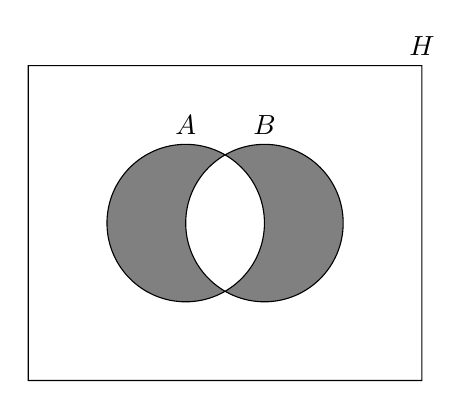
\begin{tikzpicture}[fill=gray]
            % left hand
            \scope
            \clip (-2,-2) rectangle (2,2)
                  (1,0) circle (1);
            \fill (0,0) circle (1);
            \endscope
            % right hand
            \scope
            \clip (-2,-2) rectangle (2,2)
                  (0,0) circle (1);
            \fill (1,0) circle (1);
            \endscope
            % outline
            \draw (0,0) circle (1) (0,1)  node [text=black,above] {$A$}
                  (1,0) circle (1) (1,1)  node [text=black,above] {$B$}
                  (-2,-2) rectangle (3,2) node [text=black,above] {$H$};
        \end{tikzpicture}
    \end{center}
    This diagram perfectly represents the overlap between the two sets.
    If you caught it earlier, what we're actually finding is $A\cup B$.
    The Inclusion\textemdash Exclusion Principle is merely a way of finding it algebraically.
    The image above represents the equation below.
    \begin{equation*}
        |A\cup B| = |A| + |B| - |A\cap B|
    \end{equation*}
    What happens if we have have three events we need to find the union of though?
    To do that, we'll follow the same principles, and use the equation below.
    \begin{equation*}
        |A\cup B\cup C| = |A| + |B| + |C| - |A\cap B| - |A\cap C| - |B\cap C| + |A\cap B\cap C|
    \end{equation*}
    %%TODO: Include a Venn Diagram for this equation above.

\section{Modelling with Matrices}
    
    \subsection{Intro to Matrices}
    A matrix is a rectangular array of numbers that is used to organize data.
    If you are used to computer programming, you will recognize them as 2D arrays.
    If you are good with set notation, they are in essence, a set of sets.
    Matrices follow the format below:
    \begin{equation*}
        X =
        \begin{bmatrix}
            a & b & c \\
            d & e & f
        \end{bmatrix}
    \end{equation*}
    Matrices have various properties, and unique terms created to describe them.
    For instance, looking at the matrix above, we can safely say that $a$ in an entry, as defined below.
    \begin{definition}
        Entry: An entry refers to a number in a matrix.
    \end{definition}
    How did we figure out the number of entries in the matrix? Simple, we can use the matrix's \emph{dimensions} to figure that out.
    \begin{definition}Dimensions:
        These refer to the size of the matrix, described by the number of rows and columns.
        The formula below is used to solve for dimensions, where D is the result, $R$ is the rows, and $C$ is the columns.
        \begin{equation*}
                D = R \cdot C
        \end{equation*}
    \end{definition}
    Matrix's entries are numbered in a way so that it is easy to refer to a specific entry.
    Capital letters are used for the names of matrices, and lowercase characters are used for the names of entries.
    Shown below are the entries named, with numbers instead of letters.
    The first character represents the y value, whereas the second represents the x value.
    In the equation below, $a_{13}$ represents the entry in row 1, column 3.
    \begin{equation*}
        X =
        \begin{bmatrix}
            a_{11} & a_{12} & a_{13} \\
            a_{21} & a_{22} & a_{23}
        \end{bmatrix}
    \end{equation*}
        
    \subsection{Variations and Classifications of Matrices}
    Matrices can be transformed, and compared to each other, much like sets.
    The definitions of the variations and classifications of the matrices are listed below.
    \begin{definition}Transpose Matrix: 
        A transpose matrix is a matrix obtained by interchanging the rows and columns. This is written as $X^{+}$. Shown below is Matrix W, and the transposed equivalent.
        \begin{equation*}
            W =
            \begin{bmatrix}
                a & b & c \\
                d & e & f
            \end{bmatrix}
            -> X^{+} =
            \begin{bmatrix}
                a & d \\
                b & e \\
                c & f
            \end{bmatrix}
        \end{equation*}
    \end{definition}
        
    \begin{definition}Column Matrix:
        A Column Matrix is a matrix that has only one x value. Instead of rows and columns, it is merely a column.
        For instance, Matrix X in this case would be a Column Matrix.
        \begin{equation*}%Column Matrix
            X =
            \begin{bmatrix}
                a&\\
                b&\\
                c
            \end{bmatrix}
        \end{equation*}
    \end{definition}
        
    \begin{definition}Row Matrix:
        A Row Matrix is a matrix that has only one y value. It is the transpose of the Column Matrix For instance, Matrix Y in this case would be a Row Matrix.
        \begin{equation*}%Row Matrix
            Y =
            \begin{bmatrix}
                a & b & c
            \end{bmatrix}
        \end{equation*}
    \end{definition}
        
    \begin{definition}Square Matrix:
        A Square Matrix is a matrix in which the rows and columns are equal.
        For instance, Matrix Z below is a Square Matrix.
        \begin{equation*}%Column Matrix
            Z =
            \begin{bmatrix}
                a & b & c\\
                d & e & f\\
                g & h & i
            \end{bmatrix}
        \end{equation*}
    \end{definition}
        
    \subsection{Basic Operations with Matrices}
        Matrices may only be added or subtracted when they have the same dimensions.
        Adding matrices is done by adding entry by entry to the other matrix.
        $A_{12}$ will be added with $B_{12}$ and so forth.
        Shown below is a valid example of adding with matrices in which the entries are labeled to show proper addition:
        \begin{equation*}
            \begin{bmatrix}
                a_{11} & a_{12} & a_{13} \\
                a_{21} & a_{22} & a_{23}
            \end{bmatrix}
            +
            \begin{bmatrix}
                b_{11} & b_{12} & b_{13} \\
                b_{21} & b_{22} & b_{23}
            \end{bmatrix}
            =
            \begin{bmatrix}
                (a+b)_{11} & (a+b)_{12} & (a+b)_{13} \\
                (a+b)_{21} & (a+b)_{22} & (a+b)_{23}
            \end{bmatrix}
        \end{equation*}
        They may also be multiplied by a coefficient, by multiplying the coefficient with every entry in the matrix.
        Shown below is a proper solution in which a matrix is multiplied by a coefficient, with entries labeled:
         \begin{equation*}
            x
            \begin{bmatrix}
                y_{11} & y_{12} & y_{13} \\
                y_{21} & y_{22} & y_{23}
            \end{bmatrix}
            =
            \begin{bmatrix}
                xy_{11} & xy_{12} & xy_{13} \\
                xy_{21} & xy_{22} & xy_{23}
            \end{bmatrix}
        \end{equation*}
        
    \subsection{Multiplying Matrices Together}
        Matrices may also be multiplied with other matrices, yet to do so we must follow certain rules.
        Let's say we have Matrix A and Matrix B as shown below.
        To multiply, we need to make sure the \emph{inner dimensions} are the same.
        We know that Matrix A's dimensions are $3 \cdot 2$, whereas for Matrix B, they are $2 \cdot 3$.
        Since we know this, we can find the \emph{inner dimensions}.
        The \emph{inner dimensions}, equals the columns of Matrix A and the rows of Matrix B.
        In this case, that would work out to be $3$ and $3$.
        Since they are the same, we are allowed to multiply these matrices. 
        \begin{equation*}%Demonstrating Matrices. 
            A =
            \begin{bmatrix}
                a & b & c\\
                d & e & f\\
            \end{bmatrix}
            B = 
            \begin{bmatrix}
                u & v\\
                w & x\\
                y & z
            \end{bmatrix}
        \end{equation*}
        Next, the rows of Matrix A times the columns of Matrix B, also known as the \emph{outer dimensions}, will give us the dimensions of the resultant matrix.
        Since Matrix A has two rows, and Matrix B has two columns, our resultant Matrix will possess the dimensions $2\cdot2$.
        Shown below is the updated equation. 
        \begin{equation*}
            \begin{bmatrix}
                a & b & c\\
                d & e & f\\
            \end{bmatrix}
        \cdot
            \begin{bmatrix}
                u & v\\
                w & x\\
                y & z
            \end{bmatrix}
            =
            \begin{bmatrix}
                ?&?\\
                ?&?
            \end{bmatrix}
        \end{equation*}
        Multiplying them is a bit strange at first, because to do it, we multiply row by row.
        Starting at the first row in Matrix A, we can see we have $a_{11},b_{12},c_{13}$ as our values, with their locations being labeled for convenience.
        We must multiply these values each column in Matrix B, starting with the values $u_{11},w_{21},y_{31}$.
        To find entry (1,1) we can use the formula shown below, where $E$ represents the entry, $r$ represents a row in Matrix A, and c represents a column in Matrix B.
        \begin{equation*}
            E_{11} = r_{11} \cdot c_{11}  +  r_{12} \cdot c_{21}  +   r_{13} \cdot c_{31}
        \end{equation*}
        If you want to do it just by eye, you can multiply $A_{11}$ by $B_{11}$, $A_{12}$ by $B_{21}$, and $A_{13}$ by $B_{31}$, and add them all up.
        It will seem totally awful at first, but after you do a couple it'll all work out fine.
        
    \subsection{Identity Matrices}
        An Identity Matrix is a $n\cdot n$ size matrix in which every number along the main diagonal is a 1, and the rest are zeros.
        Shown below is Matrix I, a $3\cdot 3$ Identity Matrix.
        \begin{equation*}
        I =
            \begin{bmatrix}
                1 & 0 & 0\\
                0 & 1 & 0\\
                0 & 0 & 1
            \end{bmatrix}
        \end{equation*}
        This matrix is very special, as any square matrix multiplied by its inverse will equal an Identity Matrix.
        We can further formalize this assumption, by referring to a given matrix as Matrix A.
        \begin{equation*}
            A\cdot A^{-1} = I
        \end{equation*}
        Its too bad we can't divide matrices, how can we ever solve for I now? Good thing we can use something called an Inverse Matrix.
        
    \subsection{Finding Inverse Matrices}
        Finding the inverse of large matrices is one of the most mathematically intensive processes out there.
        Good thing we'll only be finding the inverse of a $2\cdot2$ matrix instead. To find the inverse of a $2\cdot 2$ matrix, we must use first define the matrices.
        \begin{equation*}
        A = 
            \begin{bmatrix}
                a & b\\
                c & d
            \end{bmatrix}
        \end{equation*}
        Now that we have the starting matrix, it is time to find the inverse. To find it, we must multiply the determinant, by the matrix, and swap several spots of numbers. Again, sounds odd, but we just need to follow the formula below.
        \begin{equation*}
        A^{-1} = \frac{1}{ad-bc}
            \begin{bmatrix}
                d & -b\\
                -c & a
            \end{bmatrix}
        \end{equation*}
        After this step, simply multiply the determinant into the matrix, and you have found $A^{-1}$!

\section{Probability}

    \subsection{What is probability?}
    Probability is the measurement of the chance of an event occurring.
    If you've ever checked the weather and seen that it's a "20\% chance of rain", you've seen probability in action.
    To start, we'll need to define some terms.
    \begin{definition}
        Outcomes: A possible result, typically referencing all of the possible results from the situation.
    \end{definition}
    \begin{definition}
        Events: These typically refer to desired outcomes
    \end{definition}
    Typically when finding probability, we'll divide all possible outcomes from our desired outcomes.
    Thinking in terms of set notation, we'll refer to all of our desired outcomes as n(A), where A is our desired outcome.
    n(S) will refer to all of the possible outcomes, and P(A) referring to the likelihood of A occurring.
    To generalize, we'll use the equation below.
    \begin{equation*}
        P(A) = \frac{n(A)}{n(S)}
    \end{equation*}
    Since the number of desired outcomes will never be greater than the number of total outcomes, we'll always have a decimal between 0 (0\%) and 1 (100\%), which we can convert to a percentage (ex. $\frac{1}{4}=0.25=25\%$), though typically we'll simply leave it as a reduced version of the fraction.
    
    \subsection{Mutually Exclusive Events and Non-Mutually Exclusive Events}
    Mutually Exclusive events are events that have zero overlap with other events.
    Recall the Venn Diagram of Sets in the Combinations section, and assume A and B are both events.
    To find the probability of either of them happening, we'll have to remember the equation:
    \begin{equation*}
        n(A\cup B) = n(A) + n(B)
    \end{equation*}
    This equation finds all the ways A or B can happen, with zero overlap.
    The problem with this equation is that it only finds the number of wanted outcomes.
    Remember, to find the probability of something, we find the wanted outcomes, and divide it by all of the possible outcomes.
    After this, our equation will look like this:
    \begin{equation*}
        \frac{n(A \cup B)}{n(S)} = \frac{n(A) + n(B)}{n(S)}
    \end{equation*}
    Which reduces to:
    \begin{equation*}
        P(A\cup B) = P(A) + P(B)
    \end{equation*}
    For non-mutually exclusive events, we must instead use a different equation, more accurate to the one we've discussed in the Sets Unit.
    Following the same logic we used earlier, our equation works out to:
    \begin{equation*}
        P(A\cup B) = P(A) + P(B) - P(A\cap B)
    \end{equation*}
    Where $P(A\cap B)$ equals the probability of both of those events occurring.

    \subsection{Independent Probability}
    When two events occur at the same time, or one after another with no effect on each other, they are called Independent Events.
    If you roll a die, then select a card, this would be independent, as the outcomes don't affect each other.
    So solve an Independent Probability question we'll have to think in terms of sets, so the probability of A and B, can be solved with the equation below.
    \begin{equation*}
        P(A\cap B) = P(A) \cap(B)
    \end{equation*}
        But what happens if we need to find the probability of $(A \mbox{ or } B)$?
        To find that we'll need to use another equation.
    \begin{equation*}
        P(A\cup B) = P(A) + P(B) - P(A\cap B)
    \end{equation*}
    
    \subsection{Markov Chains}
    Markov Chains are ways of predicting probability after successive iterations.
    Suppose that Product A has a 70\% chance of repurchasing, and Product B has a 70\% chance of repurchasing, how would we model this? We'd use a Markov Chain. Shown below is our probability matrix.
    \begin{equation*}
        P = 
        \begin{bmatrix}
            0.7 & 0.3\\
            0.3 & 0.7
        \end{bmatrix}
    \end{equation*}
    Now, we have to find the initial probability of something, which we call a \textbf{transition matrix}. We'll represent this in the form of how many people started buying A or B, (shown below). Since this is the initial time, we'll refer to it as $S_{0}$, though you may also hear it called a \textbf{probability vector}.
    \begin{equation*}
    S_{0} = 
        \begin{bmatrix}
            0.6 & 0.4
        \end{bmatrix}
    \end{equation*}
    To find the next probability vector, or $S_{1}$, we'll have to multiply the transition matrix by the probability vector.
    \begin{equation*}
        \begin{bmatrix}
            0.6 & 0.4
        \end{bmatrix}
        \cdot
        \begin{bmatrix}
            0.7 & 0.3\\
            0.3 & 0.7
        \end{bmatrix}
        =
        \begin{bmatrix}
            0.54 & 0.46
        \end{bmatrix}
        = S_{1}
    \end{equation*}
    Much like rolling a die, the more times you repeat this process, the closer you are to the actual results. Though what if there was an easier way to do this?
    
    \subsection{Steady State Vectors}
    In Markov Chains, the probability vectors will eventually stop changing.
    A probability vector that remains unchanged upon multiplication is called the \textbf{steady state vector}.
    This vector will represent the long term trend of the event.
    To find this without repeating the Markov Chain multiplication, we must think of the problem in terms of a system of equations.
    \begin{equation*}
        \begin{bmatrix}
            a & b
        \end{bmatrix}
        \cdot
        \begin{bmatrix}
            0.7 & 0.3\\
            0.3 & 0.7
        \end{bmatrix}
        =
        \begin{bmatrix}
            a & b
        \end{bmatrix}
    \end{equation*}
    To have a systems of equations from this, we must first assert that $a + b = 1$, and find the other by multiplying for one of the values.
    In this case, we can see that $0.7a + 0.3b = a$.
    Now solve this systems of equations like you have done in Grade 9.
    
    \subsection{Odds}
    Have you ever heard the (seemingly wrong) Roll Up The Rim odds?
    They claim that 1 in 5 people are winners!
    But what does this mean?
    Odds are the degree of confidence that someone has that an event will occur.
    To find the odds of something occurring, we must use the formula below.
    \begin{equation*}
        P(A) : P(A)' 
    \end{equation*}
    This equation represents a ratio of the probability of A happening, against the probability of A \textbf{not} happening. Likewise with the odds of something \textbf{not occurring}, we can use the reverse of this formula.
    \begin{equation*}
        P(A)' : P(A)
    \end{equation*}
    What happens if we want to win a bet though? You've probably heard of betting odds before. To do that, we'll use the equation below, where X will equal the amount won.
    \begin{equation*}
        \frac{P(A)}{P(A)'} = \frac{\emph{Amount Bet}}{x}
    \end{equation*}
    After this, isolate X, which will give you the following equation.
    \begin{equation*}
        X = \emph{Amount Bet}\cdot\frac{P(A)'}{P(A)}
    \end{equation*}

\section{Probability Distributions}

    \subsection{What is a probability distribution?}
    A probability distribution is a method of displaying data that displays the probabilities of every possible outcome. We'll need to define a few types of distributions first though, which are uniform and non-uniform distributions.
    \begin{definition}
        Uniform Distribution: A distribution is called uniform when all of the outcomes are equally likely, just like a single die roll.
    \end{definition}
    \begin{definition}
        Non-Uniform Distribution: A distribution is called non-uniform when not all of the outcomes are equally likely, just like rolling the sum of a pair of dice.
    \end{definition}
    The variable we measure when calculating these, is called the random variable, and is denoted as $X$. The various possibilities for $X$ are the outcomes, denoted $x$. We'll typically find the probability distributions that rely on two different types of variables: discrete and continuous variables. 
    \begin{definition}
        Discrete Variables: These are values that are typically separate from each other, and have a finite number of possibilities.
    \end{definition}
    \begin{definition}
        Continuous Variables: These are values that have an infinite number of possibilities, such as a length of time.
    \end{definition}
    
    \subsection{Sigma Notation \& Regular Probability Distributions}
    Sigma Notation, or $\sum_{}^{}$, may look terrifying, but it simply means the sum of a lot of numbers. We use this when finding an expected value of something, which we'll denote as $E(x)$. To find this, we'll use the equation below.
    \begin{equation*}
        E(x) = \sum_{i=1}^{n}x_{i}P(x_{i})
    \end{equation*}
    To break it down, the $i=1$ is the start, the $n$ is the stop, $x_{i}$ is the outcome, and $P(x_{i})$ is the possibility of that outcome.
    To show this in action, let's suppose that in a game, you'll get the amount of points you'll roll on a die.
    To find that, we'll need to use find $E(x)$.
    We know that the probability of rolling each number is $\frac{1}{6}$, and we know all the outcomes, so let's fill out the equation. First, we'll need to set our limits though.
    \begin{equation*}
        E(x) = \sum_{i=1}^{6}
    \end{equation*}
    This means that we must repeat the $x_{i}P(x_{i})$ starting at one, going to six, which would be six times.
    Now we'll expand that below.
    \begin{equation*}
        E(x) = 1(\frac{1}{6}) + 2(\frac{1}{6}) + 3(\frac{1}{6}) + 4(\frac{1}{6}) + 5(\frac{1}{6}) + 6(\frac{1}{6})
    \end{equation*}
    We can also simplify this, as we know it is a uniform distribution. Shown below is the updated equation for this uniform distribution.
    \begin{equation*}
        E(x) = \frac{1}{6}(1 + 2 + 3 + 4 + 5 + 6)
    \end{equation*}
    
    \subsection{Binomial Distribution}
    Remember binomials from combinations? They look like this $\binom{x}{y}$, and come in handy when working with distributions.
    We have to mention something called a Bernoulli Trial first.
    \begin{definition}
        Bernoulli Trials: This refers to repeated, independent trials that are measured in terms of success, or failure (or other Boolean outcomes).
    \end{definition}
    The probability distribution of the number of successes in Bernoulli Trials is called a binomial distribution, and is found using the equation below.
    \begin{equation*}
        P(x) = \binom{n}{x}p^{x}q^{n-x}
    \end{equation*}
    The equation solves for the probability of exactly $x$ successful trials out of $n$ total trials. In this equation, $p$ represents the probability of success, and $q$ represents the probability of failure.
    To find the expected value for a binomial distribution, we'll resort to using the formula below.
    \begin{equation*}
        E(x) = n\cdot p
    \end{equation*}

    \subsection{Geometric Distributions}
    A geometric distribution is found when an experiment is repeated just \textbf{until the first success}.
    It differs from binomial distributions, as the number of trials is not known at the start. 
    Just before the success, there is something called a "waiting period". 
    \begin{definition}
        Waiting Period: This is the number of failures before the first and only success. 
    \end{definition}
    If you have 8 failures before your success, then you have a waiting period of 8.
    To solve for the probability of success after $x$ failures, we can use the formula below.
    Remember, $x$ represents the waiting period.
    \begin{equation*}
        P(x) = q^{x}p^{1}
    \end{equation*}
    In this equation, the variable $p$ \textbf{must have a max of one} as you can never have more than one success in a Geometric Distribution. To find your expected waiting period, you must solve for $E(x)$, which you can do by using the formula below.
    \begin{equation*}
        E(x) = \frac{q}{p}
    \end{equation*}
    \subsection{Hyper\textemdash Geometric Distribution}
    Hyper-Geometric Distribution are quite similar to Geometric Distributions, yet they are dependent, rather than independent.
    Repeated sampling without replacement exhibits this type of process.
    To find the probability of this, we must use the equation below, where $n$ represents the total number of choices,
    $r$ represents the total number of items chosen,
    $a$ represents the number of successes to choose from, and
    $x$ represents the successes chosen.\\
    \begin{equation*}
        P(x) = \frac{\binom{a}{x}\cdot \binom{n-a}{r-x}}{\binom{n}{r}}
    \end{equation*}
    We can also find the number of expected successes chosen by using the formula below, using the same variables as in the equation above.
    \begin{equation*}
        E(x) = r \cdot \frac{a}{n}
    \end{equation*}
    
\section{Single Variable Statistics}
    
    \subsection{Intro to Statistics}
    This is a massive shift compared to the rest of the stuff we've done so far. It is a lot of (relatively simple) graphing, and data management, and also includes a lot of spreadsheet work (which I may or may not include). Using a frequency table will help you, as well as attention to detail.
    
    \subsection{Displaying Frequency}
    To start, we're going to have to (re)define some stuff you have learned in earlier years. This will seem like a lot at first, but most of it is quite basic, and there are no equations to memorize.
    \begin{definition}
        Range: A range, in relation to sets of data, is how far apart the data points are spread. It is calculated by taking the largest number, and subtracting it by the smallest. 
    \end{definition}
    \begin{definition}
        Frequency Diagram: A frequency diagram is a graph used to show the frequency of various points, or intervals of data (ex. years, or decades). 
    \end{definition}
    \begin{definition}
        Frequency Polygon: A shape that helps the reader understand the overall shape of the diagram or distribution.
    \end{definition}
    \begin{center}
        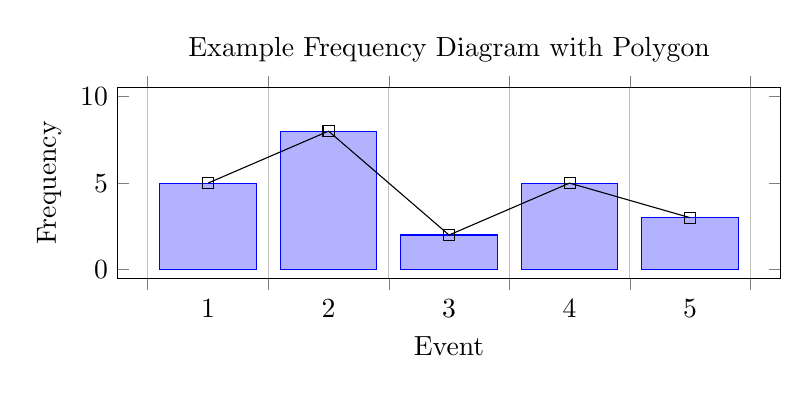
\begin{tikzpicture}
            \begin{axis}[
                width=10cm,
                height=4cm,
                x tick label style={
                	/pgf/number format/1000 sep=},
                title=Example Frequency Diagram with Polygon,
                ylabel=Frequency,
                xlabel=Event,
                ymin=0,
                ymax=10,
                xmin=1,
                xmax=6,
                enlargelimits=0.05,
                ybar interval=0.8,
            ]
            \addplot
                coordinates {
                    (1,5)
                    (2,8)
                	(3,2)
                	(4,5)
                	(5,3)
                	(6,0.0000)};
            \addplot[sharp plot,mark=square]
                coordinates {
                    (1.5,5)
                    (2.5,8)
                	(3.5,2)
                	(4.5,5)
                	(5.5,3)};
            \end{axis}
        \end{tikzpicture}
    \end{center}
    \begin{definition}
        Cumulative Frequency: This refers to the running total of frequencies. Shown below is an example of once such diagram.
    \end{definition}
    \begin{center}
        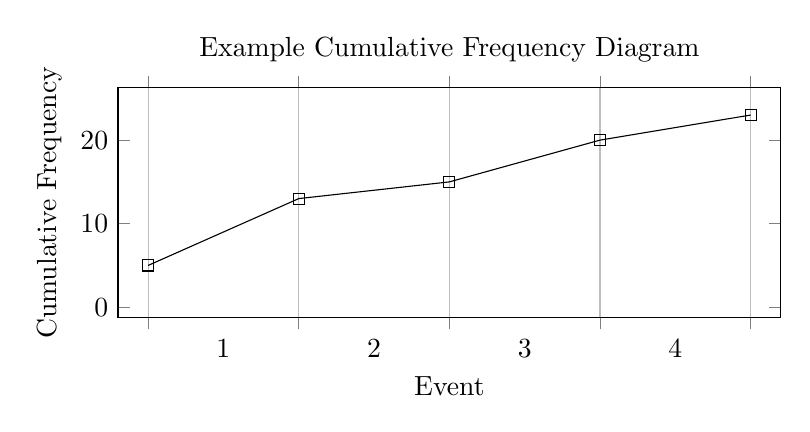
\begin{tikzpicture}
            \begin{axis}[
                width=10cm,
                height=4.5cm,
                x tick label style={
                	/pgf/number format/1000 sep=},
                title=Example Cumulative Frequency Diagram,
                ylabel=Cumulative Frequency,
                xlabel=Event,
                ymin=0,
                ymax=25,
                xmin=1,
                xmax=5,
                enlargelimits=0.05,
                ybar interval=1,
            ]
            \addplot[sharp plot,mark=square]
                coordinates {
                    (1,5)
                    (2,13)
                	(3,15)
                	(4,20)
                	(5,23)
                };
            \end{axis}
        \end{tikzpicture}
    \end{center}
    \begin{definition}
        Relative Frequency: This means the frequency expressed as a percentage, found by dividing the frequency by the total number of results.
    \end{definition}
    \begin{center}
        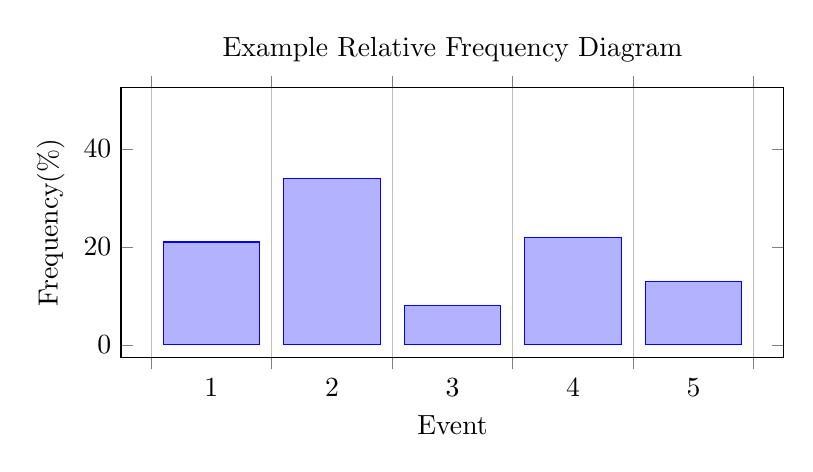
\begin{tikzpicture}
            \begin{axis}[
                width=10cm,
                height=5cm,
                x tick label style={
                	/pgf/number format/1000 sep=},
                title=Example Relative Frequency Diagram,
                ylabel=Frequency(\%),
                xlabel=Event,
                ymin=0,
                ymax=50,
                xmin=1,
                xmax=6,
                enlargelimits=0.05,
                ybar interval=0.8,
            ]
            \addplot
                coordinates {
                    (1,21)
                    (2,34)
                	(3,8)
                	(4,22)
                	(5,13)
                	(6,0.0000)};
            \end{axis}
        \end{tikzpicture}
    \end{center}
    \begin{definition}
        Histogram: Essentially a bar graph, yet with the data in groupings, instead of being separate.
    \end{definition}
    \begin{center}
        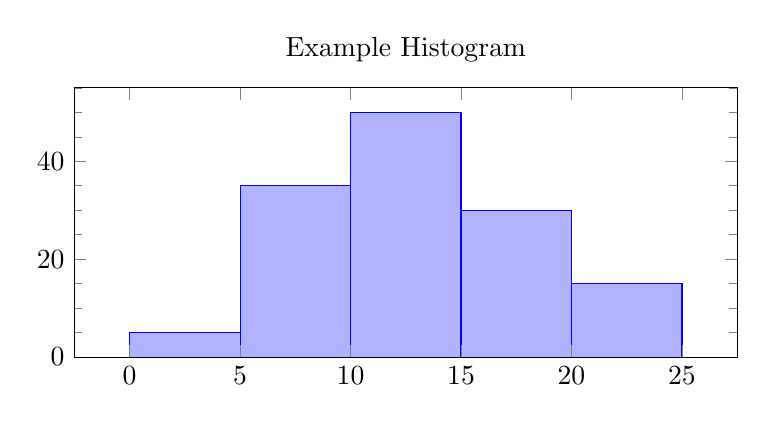
\begin{tikzpicture}
            \begin{axis}[
                x tick label style={
                	/pgf/number format/1000 sep=},
                title=Example Histogram,
                width=10cm,
                height=5cm,
                ymin=0,
                ymax=55,
                minor y tick num = 3,
                area style,
            ]
            \addplot+[ybar interval,mark=no] plot coordinates {
                (0, 5)
                (5, 35)
                (10, 50)
                (15, 30)
                (20, 15)
                (25, 0)};
            \end{axis}
        \end{tikzpicture}
    \end{center}
    All of this data and results above can be displayed and organized in something called a frequency table, as defined, and shown below.
    \begin{definition}
        Frequency Table: This is a table that contains all of the above results, as well as tallies of data points.
    \end{definition}
    \begin{center}
        \begin{tabular}{ | l | l | l | l |}
            \hline
            (x) & Frequency & Relative Frequency & Cumulative Frequency \\ \hline
            1 & 5 & $\frac{5}{23}$=21\% & 5 \\ \hline
            2 & 8 & $\frac{8}{23}$=34\% & 13 \\ \hline
            3 & 2 & $\frac{2}{23}$=8\% & 15 \\ \hline
            4 & 5 & $\frac{5}{23}$=22\% & 20 \\ \hline
            5 & 3 & $\frac{3}{23}$=13\% & 23 \\ \hline
        \end{tabular}
    \end{center}
    
    \subsection{Measures of Central Tendency}
    Measures of Central Tendency deal with the various numbers we use to find data points we can make assumptions based on.
    These three numbers we use are called the \textbf{mean, median and mode}.
    \begin{definition}
        Mean: The mean represents the average of the data, and is found by using the equation below.
        \begin{equation*}
            \mean{x} = \frac{\sum x}{n}
        \end{equation*}
    \end{definition}
    \begin{definition}
        Median: The median represents the middle-most point of data, for example in a set of 5 integers, the median will be the third.
        To find the median of an list of data of which \textbf{n is odd numbered} you can use the equation below.
        \begin{equation*}
            \median{x} = \mbox{\emph{Number in middle of data}}
        \end{equation*}
        if the equation is even numbered, you must use the average of the numbers that the median is in between.
        For example if you have a list of 8 numbers, the median would be the average of 4 and 5.
        The equation for this can be seen below.
        \begin{equation*}
            \median{x} = \frac{\mbox{\emph{Left Number + Right Number}}}{2}
        \end{equation*}
    \end{definition}
    \begin{definition}
        Mode: The mode represents the data point that has been repeated the most often. Can be found by merely looking at the highest repeated data set.    
    \end{definition}
    
    \subsection{Measures of Spread}
    A measure of spread is a measurement that describes how the data is distributed, and how widely it fluctuates.
    To measure these, we divided the spread of the data into something called \emph{quartiles.}
    A quartile, just like its name implies, is merely a quarter of the data.
    The first Quartile (referred to henceforth as Q1) is the median of the \textbf{FIRST HALF} of the data, Q2 is the middle (or median), and Q3 is the median of the \textbf{LAST HALF} of the data.
    If we want to find the most relevant data, we'll typically look at the data between Q1 and Q3, this range of data is called the Inter Quartile Range (IQR).
    \begin{definition}
        Inter Quartile Range: This is the middle-most data, and a grouping you can easily make assumptions from. To find this, we use the equation below.
        \begin{equation*}
            \mbox{IQR} = \mbox{Q3}-\mbox{Q1}
        \end{equation*}
    \end{definition}
    Using this, we can also find other data to make assumptions off of, such as the Semi-Inter Quartile Range.
    \begin{definition}
        Semi Inter Quartile Range: This is $\frac{1}{2}$ of the difference of the IQR, and therefore is less affected by outliers. Can also be referred to as the SIQR, and is found by the equation below.
        \begin{equation*}
            \mbox{SIQR} = \frac{\mbox{IQR}}{2}
        \end{equation*}
    \end{definition}
    We can display these using something called a \textbf{box and whisker plot}.
    This will show Q1, Q2, and Q3, along with the highest and lowest datum.
    An example of this is shown below.
    \begin{center}
        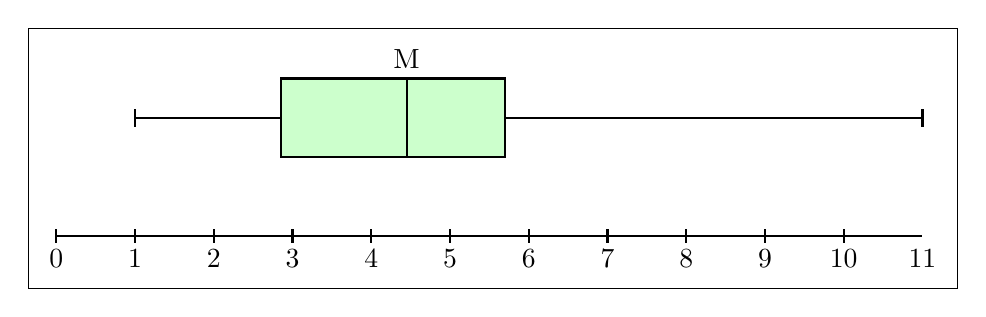
\begin{tikzpicture} [thick, framed]
            \filldraw[fill=green!20] (2.85,0) rectangle (5.7,1);
            \draw (4.45,0)--(4.45,1) node[above]{$\textsc{M}$};
            \draw (5.7,0.5)--(11,0.5);%vandret linie til max
            \draw (2.85,0.5)--(1,0.5);%vandret linie til min
            \draw (11,0.39)--(11,0.61);
            \draw (1,0.39)--(1,0.61);
            \draw [
                postaction={
                    draw,
                    decoration=ticks,
                    segment length=1cm,
                    decorate,
                }
             ] (0,-1) -- (11,-1);
             \foreach \tick in {0,...,11}
                \node at (\tick,-1) [below=1pt] {\tick};
        \end{tikzpicture}
    \end{center}
    \subsection{Intro to Variance}
    To calculate the variance, we must first calculate the deviations. 
    A deviation is the difference between an individual value in a data set and the mean of that set.
    To calculate the deviation, we'll need to use the equation below.
    \begin{equation*}
        \mbox{Deviation}= x - \mean{x}
    \end{equation*}
    We use different kinds of deviations for various reasons, such as Mean Deviations ($md$) and Standard Deviations ($\sigma$) They are defined below, though most typically we will use the Standard Deviation. Most of these can be calculated much easier if you use the \emph{STAT} mode on your calculator, but the equations will be below if your calculator doesn't support that.
    \begin{definition}
        Mean Deviation: The mean deviation is the mean of all the distances to the mean. To calculate this, we'll use the formula below to solve for $md$, which represents the mean deviation. 
        \begin{equation*}
            md = \frac{\sum|x-\mean{x}|}{n}
        \end{equation*}
    \end{definition}
    \begin{definition}
        Standard Deviation: This is more widely used, and differs from the mean deviation in the fact that it uses square roots and exponents rather than the absolute value function. Will always be bigger than the mean deviation, and is shown as $(\sigma)$. 
        \begin{equation*}
            \sigma = \sqrt{\frac{\sum(x-\mean{x})^2}{n}}
        \end{equation*}
    \end{definition}
    Once we know the deviation, we can find the variance of various numbers.
    \begin{definition}
        Variance: This number represents the average of the squares of the deviations. You can find this by simply squaring the Standard Deviation (giving you $\sigma^{2}$), or by using the equation below.
        \begin{equation*}
            Variance = \frac{\sum(x-\mean{x})^{2}}{n}
        \end{equation*}
    \end{definition}
    
    \subsection{Z\textemdash Scores}
    A Z-Score is the number of Standard Deviations that a datum is from the mean. We can find this using the equation below. 
    \begin{equation*}
        z = \frac{x-\mean{x}}{\sigma}
    \end{equation*}
    If $z<0$ the element is less than the mean, if $z=0$, the element is equal to the mean, and if $z>0$, the number is greater than the mean.
    
    \subsection{Deviations with Intervals Data}
    When data is grouped into intervals, the formula for mean deviation and standard deviation change. Mean Deviation changes to the equation below.
    \begin{equation*}
        md = \frac{\sum f|x-\mean{x}|}{n}
    \end{equation*}
    Standard Deviation also changes into the formula below.
    \begin{equation*}
        \sigma = \sqrt{\frac{\sum f(x-\mean{x})^2}{n}}
    \end{equation*}
    In both of these equations, $f$ represents the frequency of the interval. 
    
    \subsection{Chebyshev's Theorem}
    Chebyshev's Theorem states that given a set of data with a mean (designated $\mean{x}$) and a Standard Deviation ($\sigma$), then \textbf{at least} x\% of the will be within $k$ standard deviations of the mean. We find this using the equation below.
    \begin{equation*}
        x = (1-\frac{1}{k^2})\%
    \end{equation*}
    
    \subsection{Gathering Data}
    This subsection is entirely definitions, and as such is quite lengthy. It is tested on, but I believe it is multiple choice. As such this is semi-important if any research or actual studies are ever done in your class, or in the real world. 
    \begin{definition}
        Population: Refers to individuals who belong to a group being studied. 
    \end{definition}
    \begin{definition}
        Sample: A subset of a population
    \end{definition}
    \begin{definition}
        Simple Random Sample: Every member of the population has an equal chance of being selected.  
    \end{definition}
    \begin{definition}
        Systematic Sample: Selected by iterating through the population and selecting members at regular intervals.   
    \end{definition}
    \begin{definition}
        Stratified Sample: A group of population members with similar characteristics is called a stratum. A stratified sample has the same proportion of members from each stratum. 
    \end{definition}
    \begin{definition}
        Cluster Sample: When certain groups are representative of the entire population, this takes a random selection of such groups. 
    \end{definition}
    \begin{definition}
        Multistage Sample: Uses several levels of random sampling, randomly sample from groups within groups. 
    \end{definition}
    \begin{definition}
        Voluntary Response Sample: Researcher invites any member of population to participate. Results skewed as people who choose to participate not always representative of the population.
    \end{definition}
    \begin{definition}
        Convenience Sample: Easily accessible sample of the population.
    \end{definition}
    \begin{definition}
        Bias: Any factor that favors certain outcomes or responses
    \end{definition}
    \begin{definition}
        Sampling Bias: Occurs when the sampling frame does not reflect the characteristics of the population.
    \end{definition}
    \begin{definition}
        Non-response Bias: Occurs when particular groups are under-represented because they choose to not participate.   
    \end{definition}
    \begin{definition}
        Measurement Bias: Occurs when the data collection method consistently misrepresents the characteristics of a population.    
    \end{definition}
    \begin{definition}
        Response Bias: Occurs when the participants in a survey deliberately give false/misleading answers.
    \end{definition}

\section{Two-Variable-Stats}

    \subsection{Differences compared to Single Variable Stats}
    Two variable is used quite widely, and can be used to measure the effects of various things, rather than just comparing frequency as we have previously done.
    We can compared both $x$ and $y$ values, giving us a lot more freedom, but a lot more complex graphing.
    
    \subsection{Linear Correlation}
    Linear correlation is used to find relationships between two variables. 
    We plot or graph this to easier visualize the results, and relationships.
    We often use this to discern if the variations in one variable(independent) affect the other (dependant). 
    This correlation will be either known as a positive correlation, or a negative correlation. 
    \begin{definition}
        Positive Correlation: A correlation is positive if the dependant variable increases when the independent variable is increased. 
    \end{definition}
    \begin{definition}
        Negative Correlation: A correlation is negative if the dependant variable \emph{decreases} when the independent variable is increased.
    \end{definition}
    These correlations also have various \textbf{weights}, and we can use an equation to find that; but first we must define what a weight is.
    \begin{definition}
       Relationships: These relationships show how close the line of best fit is to the points. These can be either defined as weak, moderate, and strong, and can be found by using the correlation coefficient.
    \end{definition}
    Oh no! What's the correlation coefficient? Earlier, we said we can find the weight using an equation, and this equation is known as the \textbf{correlation coefficient}.
    \begin{definition}
        Correlation Coefficient: This is a measurement of how strong the correlation is between two variables. Typically designated as $r$, we can find it by using the equation below.
        \begin{equation*}
            r = \frac{n\sum xy - (\sum x)(\sum y)}{\sqrt{[n\sum x^{2}-(\sum x)^{2}][n\sum y^{2}-(\sum y)^{2}]}}
        \end{equation*}
    \end{definition}
    This correlation is always between -1 and 1.
    If it is positive, it is a positive correlation, and the opposite is true if it is a negative. 
    You can classify a relationship type by using this number, and these following inequalities.
    \begin{center}
        \begin{itemize}
            \item Strong correlation when: $\frac{2}{3} < r < 1$
            \item Moderate correlation when: $\frac{1}{3} < r < \frac{2}{3}$
            \item Weak correlation when: $0 < r < \frac{1}{3} $
        \end{itemize}
    \end{center}
    If the correlation coefficient (henceforth referred to as $r$) is not what you'd expect, you can always improve the accuracy by increasing the number of data points. Keep in mind that you also need to follow one of the commandments of statistics: 
    \begin{center}
        \large \textbf{A STRONG CORRELATION DOES NOT NECESSARY IMPLY CAUSATION.}
    \end{center}
    
    \subsection{Linear Regression}
    Regression (in general) is defined as "an analytical technique for determining a relationship between a dependant, and an independent variable".
    When two variables \emph{appear} to have a linear correlation, you can find the line of best fit. 
    When the correlation is strong (recall: when $\frac{2}{3} < r < 1$), it is easy to estimate this line, but when any other time it is nigh impossible.
    Luckily, mathematicians don't like doing difficult things, so we have an equation for this line.\\
    
    We begin with $y = mx + b$, the standard linear formula.
    For a, we use the following equation:
    \begin{equation*}
        a = \frac{n\sum xy - (\sum x)(\sum y)}{n\sum x^{2} - (\sum x)^{2}}
    \end{equation*}
    Then for b, we'll use the next equation.
    \begin{equation*}
        b = \mean{y} - a\mean{x}
    \end{equation*}
    
    \subsection{Other Types of Regressions}
    Unfortunately, not all relationships are linear, in fact most are exponential, or polynomial.
    We can define certain growths and decays as various types defined below.
    Please keep in mind they are almost all done on the graphing calculator, and as such do not need to be memorized.
    If you have taken MHF4UI or MHF3UI, you will almost certainly know what most of these are.
    \begin{definition}
        Exponential Growth/Decay: This has an $y_{int}$ of a, and an equation of:
        \begin{equation*}
            y = ab^{x}
        \end{equation*}
    \end{definition}
    \begin{definition}
        Linear Growth/Decay: This has a $y_{int}$ of b, and an equation of:
        \begin{equation*}
            y = ax+b
        \end{equation*}
    \end{definition}
    \begin{definition}
        Quadratic Growth/Decay: This has a $y_{int}$ of c, and an equation of:
        \begin{equation*}
            y = ax^{2} + bx + c
        \end{equation*}
    \end{definition}
    \begin{definition}
        Cubic Growth/Decay: This has a $y_{int}$ of d, and an equation of:
        \begin{equation*}
            y = ax^{3} + bx^{2} + cx + d
        \end{equation*}
    \end{definition}
    \begin{definition}
        Power Growth/Decay: This has a $y_{int}$ of 0, and an equation of:
        \begin{equation*}
            y = ax^{b}
        \end{equation*}
    \end{definition}
    
    \subsection{Selecting a Regression}
    To select a regression, we must take into account various factors.
    \begin{itemize}
        \item $r^{2}$: Coefficient of determination
        \item Shape of the data.
        \item Starting Value.
        \item Ending Value.
    \end{itemize}
    
    \subsection{Cause and Effect Relationships}
    The main reason correlations are useful to us is for finding evidence of a cause/effect relationship.
    \textbf{Remember: A strong correlation doesn't prove causation}. 
    There are various types and degrees of causal relationships between variables. 
    \begin{definition}
        Cause and Effect Relationships: Exists when a change in $X$ produces a guaranteed change in $Y$.
        Physical processes display this type of relationship.
    \end{definition}
    \begin{definition}
        Common Cause Factor: Exists when a factor outside of the two variables causes similar changes in the two variables. 
    \end{definition}
    \begin{definition}
        Reverse Cause and Effect Relationship: Exists when dependent and independent are reversed when establishing causality. Example: A link between coffee and high anxiety exists, but it is later revealed that anxiety leads towards coffee consumption. 
    \end{definition}
    \begin{definition}
        Accidental Relationships: A correlation exists without any causal relationship. Merely coincidence. 
    \end{definition}
    \begin{definition}
        Presumed Relationships: A correlation that does not seem to be accidental even though no other relationships are apparent. 
    \end{definition}
\end{document}

%% EOF